%------------------------------------------------------------------------------
% On the CTD Principle's Implications for the Mind
%------------------------------------------------------------------------------


%------------------------------------------------------------------------------
%	PACKAGES AND OTHER DOCUMENT CONFIGURATIONS
%------------------------------------------------------------------------------

\documentclass[11pt]{diazessay} % Font size (can be 10pt, 11pt or 12pt)
\usepackage[font=small,labelfont=bf]{caption}

%------------------------------------------------------------------------------
%	TITLE SECTION
%------------------------------------------------------------------------------

\title{\textbf{On the CTD Principle's Implications for the Mind} \\ {\vspace{5pt}\Large\itshape The Mind in a Computable Universe}} % Title and subtitle

\author{\textbf{Ozaner Hansha} \\ \textit{Ghost in the Machine Paper \#2}} % Author and Class

\date{May 15, 2019} % Date

%------------------------------------------------

\begin{document}

\maketitle % Print the title section

%------------------------------------------------------------------------------
%	ABSTRACT
%------------------------------------------------------------------------------

\begin{abstract}
	% This paper's purpose is 3-fold: 1) Explain the CTD principle and its consequences for the nature of the mind, 2) Provide rationale for believing the CTD principle, and 3) Attacking the dualist point of view as a byproduct of our evolved psychology.
	The CTD principle provides us a solid ground with which to tackle the mind-body problem in terms of computability theory. Using it, we make the case that there is no room for dualism in a totally computable universe and that further, the notion of a totally computable universe is a reasonable one, founded in contemporary science. This is opposed to the dualist point of view which, as many contemporary cognitive scientists hold and we'll argue, is a byproduct of our evolved psychology and its propensity to assign immaterial causes and agents to complex phenomena.
\end{abstract}

%------------------------------------------------------------------------------
%	ESSAY BODY
%------------------------------------------------------------------------------

\section{Introduction}
	\subsection{The CTD Principle}
		The \textbf{Church-Turing-Deutsch (CTD) Principle} is the claim that all physical phenomena can be simulated\footnote{An important qualification I am introducing is that 'simulatable' means `calculable to any desired accuracy'. This allows us to sidestep questions of continuous/discrete spacetime and other tangential topics.} on a quantum Turing machine, the more broad quantum mechanical version of a Turing machine (Deutsch 1985). We can see that this is a stronger physical version of the Church-Turing thesis which simply posits that all 'effectively calculable' functions are computable.

		Notice that the CTD principle is a mathematically well-defined and empirical claim backed by the whole of computability theory. If there exists a physical process that is \emph{not} described by a computable function (a notion concretely defined by Gödel, Church, and Turing) then the CTD principle is false. Otherwise, it's true.

		\begin{figure}[H]
			\centering
			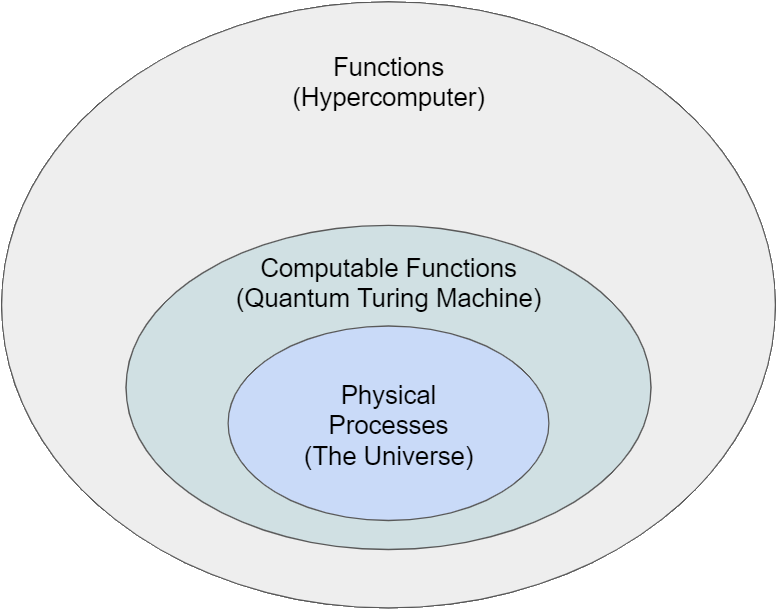
\includegraphics[width=.7\linewidth]{hierarchy.png}
			\captionsetup{justification=centering,margin=2cm}
			\caption{CTD claims that the blue circle lies entirely inside (or is equal to) the green circle.}
		\end{figure}

		While at first glance it would seem that the CTD principle lies entirely in the domain of theoretical computer science and physics, the principle actually has far reaching consequences for many problems in contemporary philosophy. In particular, the focus of this paper is its implications for the mind and its purported dualist nature.

		What does computability have to do with the human mind? Many hold, sometimes implicitly, that the human mind cannot be simulated and that a computer, a mere 'symbol manipulator' as Searle puts it, could never be conscious. This implies that the human mind is somehow `special' in its operation as all other phenomena we know of seems to be explainable via explicit computable physical principles.

	\subsection{The Consequences of CTD}
		However, such a statement cannot be thrown around lightly. Indeed, if the human mind \emph{wasn't} a totally computable physical process then it would be \textbf{uncomputable}. This means that, by definition, the human mind would be a \textbf{hypercomputer}, or at least capable of performing some sort of hypercomputation. This means that the human mind is performing a feat of computation that defies all known physics and theoretical computer science. This is a particularly far reaching consequence of a seemingly innocuous desire, as we'll argue later on, to hold on to our evolved dualist intuitions of the separation of the mind and body.
		
		And so we have an issue. Either the CTD principle is true and human minds are nothing but totally computable processes like any other physical process, or it's false and the human mind evades this attack on its dualist majesty. To a dualist inclined to believe in such superstition, the choice is clear: "CTD is false, long live the mind". But this won't be such an easy position to hold once we present several pieces of rationale in favor of CTD in the next section, or at least that's the hope.
		
		Using these rationales, we will be able to completely rule out one broad category of dualism. Other kinds of Dualism, while attacked, won't be sufficiently pushed back by the truth of the CTD principle, at least in the mind of a dualist. It will be at this point that we switch tactics and consider the cognitive science behind postulating superstitious entities, like souls or phenomenal states, in the first place.

%------------------------------------------------

\section{Reasons to Believe in the CTD Principle}
	\subsection{Quantum Algorithmic View}
		In essence, the CTD principle is equivalent to stating that all physical phenomena can be totally described by some quantum algorithm. But why would such a claim be the case? Well, according to the standard model of particle physics, all matter is composed of a finite set of fundamental particles:

		\begin{figure}[H]
			\centering
			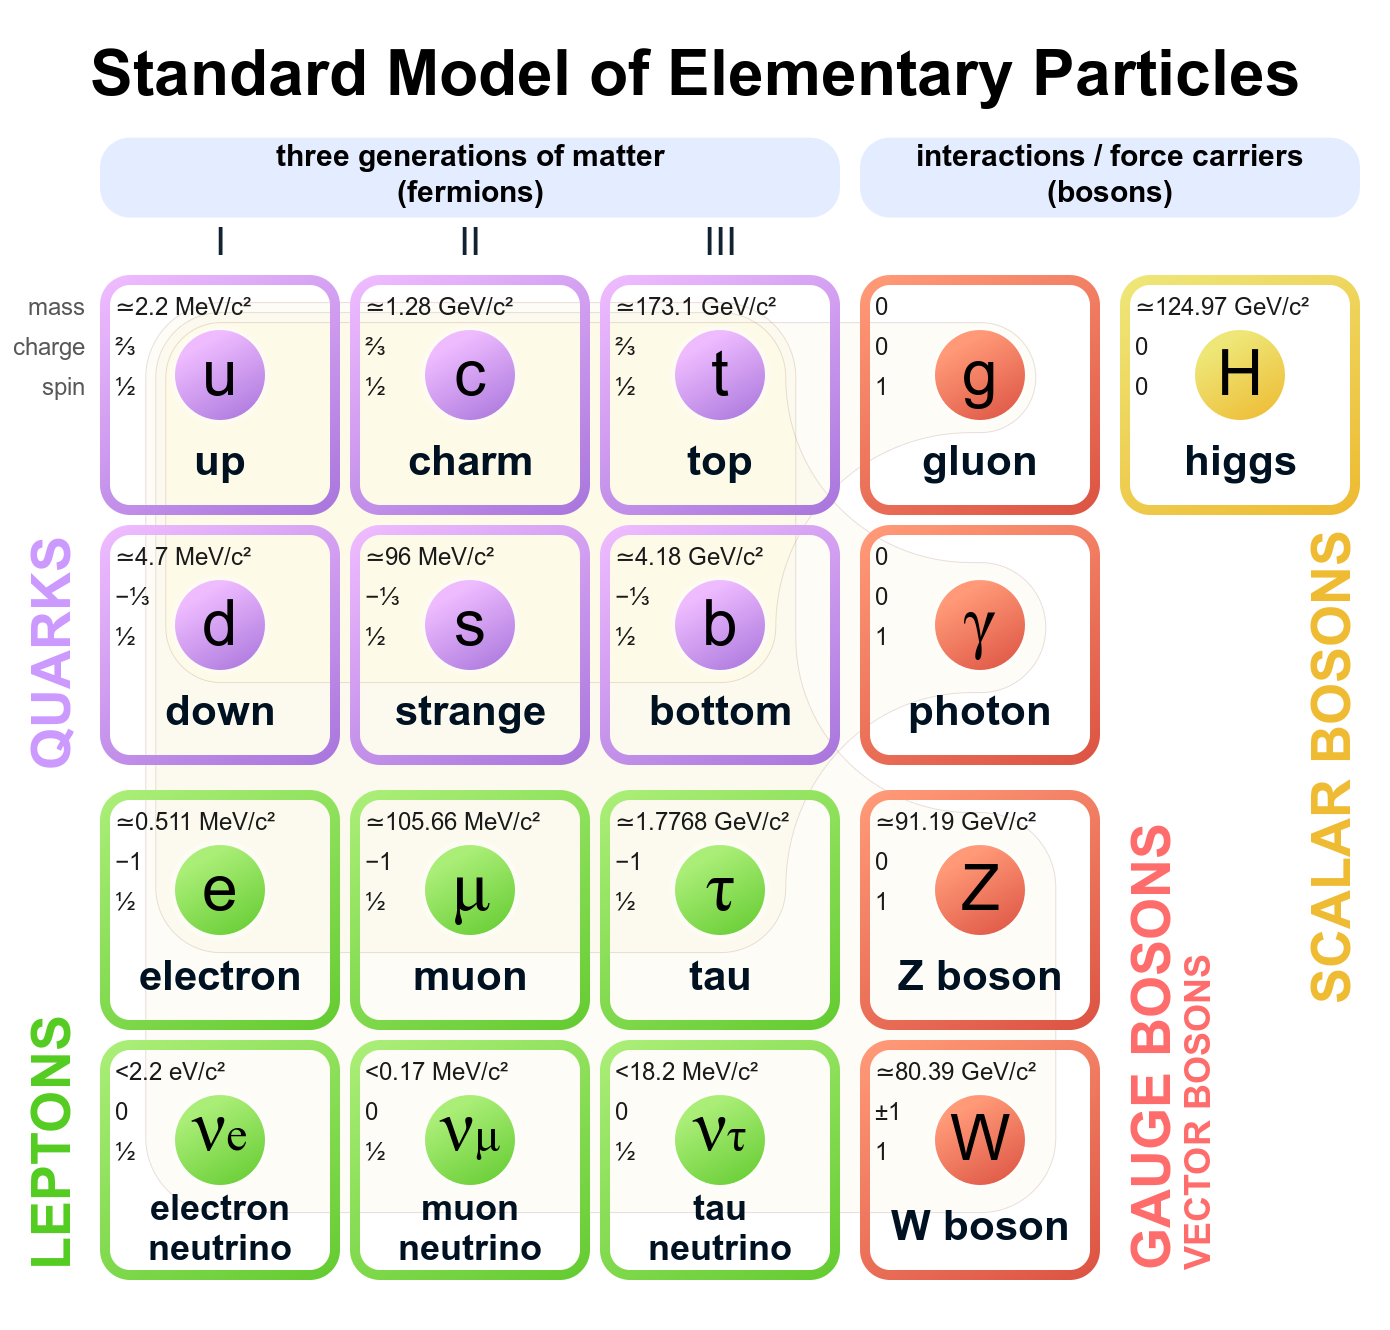
\includegraphics[width=.7\linewidth]{smpp.png}
			\captionsetup{justification=centering,margin=.7cm}
			\caption{Of these particles only 3 pertain to the atomic matter our bodies and brains are made up of: the electron and the up and down quarks.}
		\end{figure}

		The mechanics of systems of these particles are given by the laws of quantum physics. Interestingly, these laws tell us that only two broad types of action can happen to a system of quantum particles: 1) a \emph{deterministic} unitary transformation of its state, and 2) an \emph{indeterministic} collapse of its state (i.e. measurement). The latter being probabilistic and the former not.

		Why is this important? Well, all a quantum algorithm is is a series of unitary transformations and measurements of a collection of quantum particles. And since everything that any collection of matter does in this universe falls under those two categories, it too can be completely described and simulated by a quantum algorithm running on a quantum Turing machine.

		There are some technical caveats here like the fact that quantum computers are usually composed of 2-state quantum particles, or qubits, while particles in nature can have any number of states, even an uncountably infinite number ($2^{\aleph_0}$). Fortunately, this doesn't pose a problem to the definition of the CTD principle we laid out previously. This is because, with enough qubits, a quantum computer can simulate any quantum system (even one with infinite states) to any desired accuracy. Further, in principle it is possible to create quantum computer with infinite base states. That said, none of this affects the computational reach of such a machine so the point is moot.

	\subsection{Regarding Unknown Physics}
		We can see that the quantum algorithm rationale is pretty much the physicalist one in disguise, which means it still faces the same challenge: "What if there are unknown processes/matter that \emph{aren't} under the purview of quantum physics and thus may not be computable?"

		Indeed, a response a more informed dualist objector may have to the CTD principle is that our theories of the universe are known to be incomplete, e.g. what is dark matter, how does gravity work on quantum scales, etc. While it is certainly the case that the standard model does not explain all observed phenomena, to say that those as of yet unexplained phenomena are uncomputable is a much stronger statement with no backing evidence.

		It is also important to note that the regimes our known models of physics break down at are obscene. In particular, physics can totally explain the entire evolution of the universe, with no contradictions with any experimental evidence, up to $10^{-43}$ seconds (aka the Planck time) before the big bang and at scales greater than $10^{-35}$ meters (aka the Planck length). Those magnitudes are so obscenely minuscule that I don't think its possible to accurately convey said smallness. An interesting note on the Planck length is that measuring a length so small would require such high energies that the volume of space being measured would be turned into a black hole.
		
		Moreover, it has been shown that these phenomena \emph{can} be computed in principle. Take quantum gravity. String theory is a computable theory that works at sub Planck scales and does not contradict observable evidence. The reason it is not accepted, and rightly so, is that we can't test the new claims it makes with current technology (and potentially never will). But it's certainly the case that these phenomena don't exhibit some non-mathematical behavior, whatever that could possibly look like.

		This is all to say that basing one's metaphysical theory of mind on as of yet undiscovered physics or, as we'll see below, potentially undiscoverable physics, at literally unimaginable regimes of spacetime seems more like a desperate attempt to hold onto an evolved dualist intuition rather than one based in reason. We'll go into more detail on this evolved intuition once we address dualism itself.

	\subsection{The Scientific Method}
		There is also an epistemological side to believing the CTD principle. Note that all scientific theories/laws are only deemed `true' if they make testable predictions. Indeed, this is the scientific method that has netted us our understanding of the natural world. Crucial to this process, of course, is the ability to test our predictions. This ability, however, goes out the window in a world with uncomputable processes.

		Consider some phenomenon whose explanation is hypothesized to be given by some uncomputable law of physics. We would be unable to use said law to make and test predictions. There would be no way for us to use the equation/algorithm to calculate the prediction as any `effective procedure' a human could possibly perform, whether on pencil and paper or via a supercomputer, is a computable one regardless of the truth of CTD. Indeed, if we had access to a hypercomputer we might be able to avoid this, but this would require the harnessing of some uncomputable physical process to build it in the first place.
		
		It would seem that we cannot both accept that humans will one day be able to understand and have a theory of all phenomena while simultaneously believing that there is an uncomputable aspect of human consciousness. That is, unless we use a method other than science to derive facts about the physical world. I hear magic and prayer are popular candidates.

		% now of course it may be possible to have laws of physics that are accepted despite being uncomputable. We can imaigne a scenario where the behavior of a set of n particles is described by some equation. It may very well be the case that for all n less than, say, 5 are computable but for n>5 the function isn't. we may still beleive the equation holds even though we can't test it past 5.%
		
		% A better example of this is the, relativly, recent nature paper on the spectrral mass gap... of coursse this doesn't disprove CTD because the system in question is an infinite lattice of particles, something not realizable in the physical world.

	\subsection{The Existence of Hypercomputers}
		Putting aside all those reasons on why the CTD principle itself seems true, the real absurdity that a disbelief in the CTD principle entails is the existence of hypercomputers and, in our case, human beings as hypercomputers. What is a hypercomputer? A hypercomputer is a model of computation that can produce answers that an ordinary Turing machine (or even its probabilistic and quantum counterparts) could not.
		
		The problem with hypercomputers is that their existence would mean a total upturn of our notion of logic, mathematics, and the universe. Hypercomputers would allow us to solve previously undecidable problem like the halting problem or, even stranger, be able to tell whether or not a set of axioms (e.g. ZFC) is consistent or not. This is directly counter to Gödel's incompleteness theorems.
		
		These are certainly absurd consequences, doubly so since they are not products of some unavoidable evidence but of our inability to budge on our conviction of the `specialness' of human consciousness. To be fair, however, not all hypercomputers could solve these problems. It may be the case that whatever sort of hypercomputation the human mind performs, it wouldn't realize the oracle Turing machines in Turing's ordinal logic (Turing 1938) that are usually considered in discussions of hypercomputation.
		
		But this doesn't absolve the human mind. Whatever kind of hypercomputation the mind does, as a result of the negation of CTD, it will necessarily allow us to solve a class of problems previously proven to be unsolvable. Even if the brain itself is not a fully functional/programmable computer, one could in principle integrate/graft a human brain onto some normal quantum computer and use this new hybrid system to carry out said computations.
		
		Again, this is counter to many of the mathematical and physical results of the past 100 years, and in a very fundamental way. It would be as if the society we had created around us just happened to never figure this radical and reality shattering principle and all our theories and mathematical constructions just happened to work regardless.

%------------------------------------------------

\section{Room for Dualism?}
	Mind-body dualism is the view that the mental aspects of human cognition and consciousness are, in some way, non-physical. They are processes whose nature doesn't lay entirely in the observable and testable world.
	\subsection{The Four Types of Dualism}
		We can broadly split dualism into four categories based on how mental states casually interact with observable physical states:
			
		\begin{figure}[H]
			\centering
			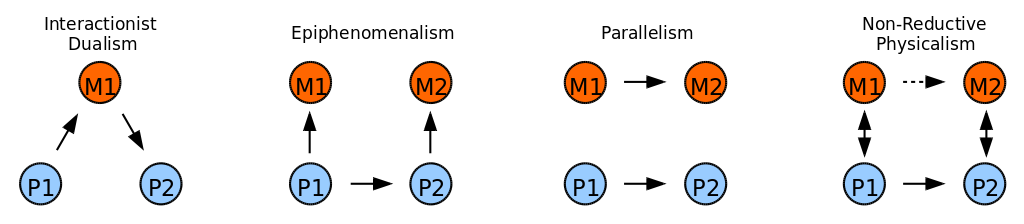
\includegraphics[width=\linewidth]{dualism.png}
			\captionsetup{justification=centering,margin=2cm}
			\caption{The blue circles are physical states and the orange mental. The arrows denote causation.}
		\end{figure}
		
		\begin{itemize}
			\item \textbf{Interactionism}: Posits that mental states can casually affect physical ones and vice versa. E.g. I eat ice cream (P1) -> I really like the flavor (M1) -> I eat more (P2).
			\item \textbf{Parallelism}: Posits that mental states just happen to correspond exactly to the physical chain of causality. I eat ice cream (P1); I really like the flavor (M1); I eat more (P2); I continue to like the flavor (M2).
			\item \textbf{Epiphenomenalism}: Posits that mental states arise from physical ones but do not interact back with the physical. That is to say, a person's actions are a product of purely physical principles, but his phenomenal experiences emerge from these states. E.g. I eat ice cream (P1) -> I really like the flavor (M1); I continue eating ice cream because the chemicals triggered a physiological reaction in my body to continue eating (P2) -> I continue to like the flavor (M2).
			\item \textbf{Non-Reductive Physicalism}: Posits that mental states are physical but not reducible to physical properties. In terms of causality, this is similar to epiphenomenalism in that mental states can't casually effect physical events (they are one and the same) but in this case they can casually effect future mental states.
		\end{itemize}
	
	\subsection{Argument by Causality}
		When it comes to interactionism, the only one of the above four in which mental states casually interact with physical states, it is easy to see that a world in which the CTD principle is true means that the physical world is \emph{causally closed} and thus there is no room for mental states to interact with the progression of physical events. A mental state changing anything about the physical chain of causality would violate the CTD principle and the laws of physics which prescribe how this chain functions.

	\subsubsection{Note on Quantum Indeterminacy}
		A particularly interesting, if not misguided, challenge a dualist might have to this is that, via the so-called `quantum randomness' present in physics, the soul/mind/whatever has a way to interact with the physical world in a casual manner. We could imagine this mental entity collapsing the quantum particles in one's brain to certain states which might have an upwards butterfly effect on the human's physical body and cause them to act in a certain way. This provides an avenue for the mental to causally affect the physical whilst, at first glance, preserving physics.
		
		Unfortunately, this is not the case. Indeed, if there was a force biasing the probabilities of the quantum particles in one's brain/body then this would be a measurable effect over many trials, violating the probabilities predicted to be the case by QM. Even though being able to empirically test one's metaphysical hypothesis leaves it in an unappealing state already, this `quantum-soul-collapse' theory also has to contend with the inability of particle collapses to affect the brain fast enough to make decisions. Even if this butterfly effect was possible via collapsing states in a certain way, the soul would have had to known ahead of time what was going to happen in order to bias the physical body to act as it had known when it was supposed to. Otherwise, it wouldn't have had enough time to make any effect on the physical body. Violating QM and causality itself are reason enough to ignore this idea.
		
		% One can imagine Getting copies of the same person to pick the same choice in some moral dilemma and have the choice depend on the superposition of a particle. If the particle goes one way he chooses A, the other B. If we make this superposition a 50-50 chance yet the soul/magical entity feels the moral choice is one or the other, the soul will bias the results making them not 50-50 and thus violating our testable hypothesis.

	\subsection{What about the Others?}
		But what about the other 3 types of dualism? Our argument by casualty doesn't seem to affect them as they posit a sort of `dual mental space' in which mental states can exist and be totally unconnected to the physical ones we see. At this point the CTD principle can only serve as a guiding principle and cannot explicitly prove the non-existence of these dual realities.
		
		\begin{wrapfigure}{r}{0.42\textwidth} % Inline image example, use an 'r' column type to position the figure on the right
			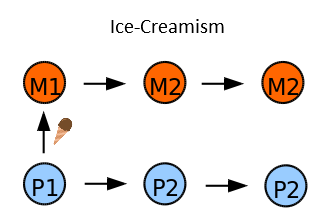
\includegraphics[width=\linewidth]{icecream.png}
			% \caption{An example fish.}
		\end{wrapfigure}

		Indeed nothing can explicitly prove their existence, as is their construction. These theories of dualism are based on no reproducible or observational evidence bar the intuition of the philosophers who conjured them up. An intuition that tells them their unshakeable feelings of a `dualist reality' must be true. Indeed, I could simply posit a new type of dualism, Ice-Creamism, in which true mental states are caused only by the consuming of ice cream, and all other mental states trace back to when one first ate ice cream. If they never ate ice cream then they never have true mental states, they are merely phenomenological zombies acting as if they are.
		
		Ridiculous to be sure, but that judgement is based not on evidence of any sort but on innate and culturally learned principles. Really any graph of mental and psychical states (blue and orange circles connected by arrows) could be a plausible theory of dualism. And as long as no orange circle connects to a blue circle, it is immune from the causality argument.
		
		And so at this point we change our strategy from arguing based on physical proof to considering why we as human beings posit such superstitious dual mental realms in the first place.

	\subsection{Natural Born Dualists}
		Cognitive scientists have long pondered why religion is such an integral part of human nature and diversity. Indeed, it seems that regardless of the place or time period, humans have always believed in some sort of superstition. Be it rain gods, angels and demons, karma, or otherwise, supernatural and superstitious beliefs seem to always take root in human societies.
	
		There are many lines of reasoning for such a phenomena. Two popular ones are:
		\begin{itemize}
			\item \textbf{Fraternity Theory}: Religions serve to build cohesion in groups, increasing their fitness, and thus are encouraged by both genetic and cultural evolution.
			\item \textbf{Opiate Theory}: Religions serve as a way to `sooth the pain of existence' (Marx 1843). By having a religion that tells us that `God has a plan for us' (i.e. afterlife, death isn't permanent) or that everybody gets what they deserve (i.e. karma), the world becomes a less unfair and scary place. These ideas produces more fit, as opposed to depressed, humans and so they spread.
		\end{itemize}
			
		But these don't cut it. Besides these theories not explaining the existence of religions and supernatural beliefs that don't build cohesion or have reassuring elements (of which many exist in non-industrialized cultures), they also don't explain why all religions have a particular aspect. Namely, why do religions need to be supernatural in nature? This is what the modern \textbf{byproduct theory} attempts to explain.
		
		Consider a stone age human trying to predict the behavior of a predator or even his fellow man. The human doesn't predict their behavior by considering the machinations of their brains and how that will cause their limbs and mouths to respond. Instead they posit an abstract mental entity associated with their body, the mind/soul, whose properties are much simpler (e.g. the lion wants to eat me -> he will probably chase me). This echoes the `voluminous predictable power' of Dennet's intentional systems theory (Dennet 1971). And indeed this is the same thing only in the context of evolutionary psychology. It would appear then that the origin of our supernatural explanations of complex phenomena (e.g. the unpredictableness of rain -> it must be the tears of a god who cries when she is disappointed in us) is an overreaction of our evolved dualist brain (Bloom 2004).
		
		In this light it becomes clear what our argument against the existence of dual mental realities is. It's that the combination of there being no ability to obtain proof of such realities, besides our own \emph{evolved} intuitions, and the fact that our evolution has biased us to believe and construct such theories in order to explain complex phenomena that we can't understand at the moment, makes for a compelling case to not trust in our intuitions regarding anything involving dualism.
		
		Indeed, this doesn't disprove dualism. It may very well be the case that non-physical dual realities do exist and we just happened to evolve in such a way as to posit their existence without proof. At this point however, it seems like a refusal of this would just be a product of our naturally dualist minds to cover for themselves.
		
		Just look at our supernatural beliefs in the past and compare them to now. Humans used to, and still do, believe in all sorts of spirits and entities to explain phenomena they didn't have the means to predict. Harvest quality? Fertility gods. Weather? Rain gods. Evil? Demons and spirits. With the introduction of monotheistic religions and God with a capital G, these explanations could remain unified under one umbrella. Slowly but surely though, we always meet these superstitions with greater understanding. In this case, using evolutionary psychology and anthropology, we have reached the point where we understand why we posited them in the first place.


	\subsection{But what about Qualia?}
		This, the hope of the physicalist, is a question to be handled by neurobiologists and psychologists. The question isn't the classical mind-body problem which seeks to explain how physical phenomena can bring about qualia, but instead why humans believe that these qualia exist in the first place. This is the job of an illusionist theory of mind (Frankish 2016).

%------------------------------------------------

\section{Conclusion}
	Summarizing, our argument has been two pronged. The main prong is highlighting the contradictions that arise from positing that there is a dual mental realm which can effect the physical one despite it, by all measures, being a computable one casually closed from such machinations. This leads to our second prong which is a response to the simple act of removing the causal power of mental states. We find that we are evolutionary prone, and for good reason, to assign immaterial mental personas and states to complex phenomena in an effort to better predict and reason about them. In light of this, we argue that our misguided attempts to construct these dualist realities are nothing but the product of an hyperactive dualist mind.

	Ultimately, the hope is that phrasing the mind-body problem in terms of computability theory sheds even more light on the absurdities of dualism. In our case, this absurdity took the form of a human brain grafted hypercomputer that violates all known results of computer science and physics. Indeed, we didn't disprove their existence but if one's metaphysical theory (which again we argue you only have because of evolutionary reasons) depends on such a bold empirical claim in the fields of theoretical computer science and quantum physics, then the theory probably isn't very appealing.

%------------------------------------------------------------------------------
%	BIBLIOGRAPHY
%------------------------------------------------------------------------------

% \bibliographystyle{unsrt}
%
% \bibliography{sample.bib}
\begin{thebibliography}{999}
\bibitem{dm}
	Turing, Alan\\
	"On Computable Numbers, with an Application to the Entscheidungsproblem", Proceedings of the London Mathematical Society, 1937
\bibitem{dm}
  Turing, Alan\\
  "Systems of Logic Based on Ordinals", Proceedings London Mathematical Society, 1938
\bibitem{dm}
	Deutsch, David\\
	"Quantum theory, the Church–Turing principle and the universal quantum computer", Proceedings of the Royal Society, 1985
\bibitem{dm}
  Nielsen, Michael\\
  "Interesting problems: The Church-Turing-Deutsch Principle", michaelnielsen.org, 2004
\bibitem{dm}
  Aaronson, Scott\\
  "Ask an unbounded question, get an uncomputable answer", www.scottaaronson.com, 2015
\bibitem{dm}
  Bloom, Paul\\
  ``Is God an Accident?", \emph{The Atlantic}, 2005
\bibitem{dm}
  Dennett, Daniel\\
  \emph{Intentional Systems}, \emph{The Journal of Philosophy}, 1971
\bibitem{dm}
  Marx, Karl\\
  \emph{Critique of Hegel's Philosophy of Right}, 1843
\bibitem{dm}
  Freud, Sigmund\\
  \emph{The Future of an Illusion}, 1972
\bibitem{dm}
  Frankish, Keith\\
  "Illusionism as a Theory of Consciousness", \emph{Journal of Consciousness Studies}, 2016
\bibitem{dm}
  Me\\
  "On Bloom's "Is God an Accident"", https://ozanerhansha.github.io/, 2019
\end{thebibliography}

%------------------------------------------------------------------------------

\end{document}
